% ============================================================================
% Accessibility
% ============================================================================
\DocumentMetadata{
  lang = en-US, 
  pdfstandard = ua-2, 
  tagging = on, 
  tagging-setup = {math/setup=mathml-SE}
}

% ============================================================================
% Document Properties - used on title slide and PDF metadata fields
% ============================================================================
\def\PresTitle{Analog Principles and Operation}  % Required - top line of title slide
\def\PresSubtitle{Programmable Logic Controllers}         % Optional - second line
\def\PresAuthor{Brad Peirson}               % Required - below dividing line
\def\PresInstitute{College of Information Technology and Engineering}       % Optional
\def\PresDate{}                             % Optional
\def\PresKeywords{}                         % Optional - used for hyperref

% Presentation Formatting
% ============================================================================
% ============================================================================
% Class Declaration
% ============================================================================
\documentclass[
        mode = handout,     % Projector = one bullet at a time, Handout = all
        font-size=14pt,     % Only accepts 9, 10, 12, 14, 17, 20
        pdfusetitle         % Pulls \title property from document
    ]
    {ltx-talk}              % ltx-talk class

% ============================================================================
% Custom Colors
% ============================================================================
\usepackage[table]{xcolor}
% Colors from the Baker College Style Guide
\definecolor{BakerADARed}{RGB}{231, 0, 46}
\definecolor{HoneyYellow}{RGB}{255, 196, 0}
\definecolor{UpNorthGreen}{RGB}{114, 191, 68}
\definecolor{LakeBlue}{RGB}{134, 183, 227}
\definecolor{BakerADI}{RGB}{58, 98, 170}
\definecolor{BakerCIM}{RGB}{217, 35, 47}
\definecolor{BakerBlack}{RGB}{31, 34, 40}
\definecolor{BakerWhite}{RGB}{255, 255, 255}
\definecolor{BakerRed}{RGB}{239, 0, 48}
\definecolor{Abbey}{RGB}{80, 82, 88}
\definecolor{RollingStone}{RGB}{121, 124, 126}
\definecolor{HitGray}{RGB}{165, 169, 172}
\definecolor{Iron1}{RGB}{201, 206, 209}
\definecolor{Iron}{RGB}{222, 225, 226}
\definecolor{BlackHaze1}{RGB}{237, 240, 240}
\definecolor{BlackHaze}{RGB}{245, 247, 247}

% ============================================================================
% Document Data
% ============================================================================
\title{\PresTitle}
\author{\PresAuthor}
\institute{\PresInstitute}
\date{\PresDate}

%Set up the hyperlink colors
\hypersetup{colorlinks,
    linkcolor=BakerBlack,
    urlcolor=BakerADARed,
    pdfauthor = {\PresAuthor},
    %pdftitle = {\PresentationTopic},   % Title is pulled directly
    pdfsubject = {\PresSubtitle},
    pdfkeywords = {\Keywords},
    pdfcreator = {LaTeX with hyperref package},
    pdfproducer = {LuaLaTeX}
    }

% Map your custom style guide colors to the progress bar aliases
\colorlet{pbcomplete}{BakerADARed}
\colorlet{pbincomplete}{Iron}

\usepackage[most]{tcolorbox}

% ============================================================================
% Footer Format
% ============================================================================
\EditInstance{footer}{std}{
  color         = Abbey,
  separator     = \hfill,
  element-order = {title, institute, framenumber},
  right-hspace  = 3mm,
  left-hspace   = 3mm,
}

% \DeclareInstance{footer}{empty}{
%   element-order = {}
% }

% ============================================================================
% Progress Bar Toggles & Helper Macros
% ============================================================================
\usepackage{xfp}        % Needed for floating point math
\newif\ifprogressbar    % Used to determine whether or not to show the bar
\progressbartrue        % Set the bar to true at the start

% Helper macro to automatically turn off the progress bar inside title/section frames
\newcommand{\makeblindframe}[1]{%
  \progressbarfalse
  #1%
  \progressbartrue
}

% ============================================================================
% Custom Page Formats
% ============================================================================
\let\oldmaketitle\maketitle         % Backup the original maketitle command
\let\oldsection\section             % Backup the original section command
\let\oldsubsection\subsection       % Backup the original subsection command

\makeatletter
\renewcommand{\maketitle}{%
\makeblindframe{%
  \disableglobalbackground
  \slidebackground{BakerPresentation_TitleBackground}%
  \color{white}%
  %\UseInstance{footer}{wallpaper}
  \begin{frame}[wallpaper]
    \vspace*{1in}%
      \begin{tcolorbox}[
          enhanced,
          colback=black,       
          colframe=black,      
          opacityfill=0.25,       
          arc=6pt,                
          boxrule=0pt,            
          left=20pt, right=20pt,  
          top=20pt, bottom=20pt,
          width=0.80\textwidth,   
          halign=left             
      ]
          \color{white}%
          % Title (Always visible)
          {\large\bfseries\sffamily \@title}\\[0.5em]%
          
          % Conditional Subtitle
          \ifx\PresSubtitle\empty
          \else
            {\normalsize\sffamily \PresSubtitle}\\[0.5em]%
          \fi
          
          % High-contrast divider line
          {\color{white!80}\rule{0.3\textwidth}{0.8pt}}\\[0.5em]%
          
          % Author (Always visible)
          {\small\sffamily \@author}\\%
          
          % Conditional Institute
          \ifx\PresInstitute\empty
          \else
            {\small\sffamily \PresInstitute}\\%
          \fi
          
          % Conditional Date
          \ifx\PresDate\empty
          \else
            {\small\sffamily \@date}\\%
          \fi
      \end{tcolorbox}%
      \vfill     
  \end{frame}%
  \enableglobalbackground{BG}%
  \color{black}%
  %\UseInstance{footer}{std}
}%
}
\makeatother

% Create a variable container to hold the current section title
\newcommand{\currentsectiontitle}{}

% Redefine \section to take 1 argument (the title)
\renewcommand{\section}[1]{%
\makeblindframe{%
  \renewcommand{\currentsectiontitle}{#1}%
  \disableglobalbackground
  \slidebackground{BakerPresentation_SectionBackground}%
  \begin{frame}
    \vfill
    %\vspace*{0.625in}%
    \begin{tcolorbox}[
        enhanced,
        colback=black,       
        colframe=black,      
        opacityfill=0.25,       
        arc=6pt,                
        boxrule=0pt,            
        left=20pt, right=20pt,  
        top=20pt, bottom=20pt,
        width=0.80\textwidth,   
        halign=left             
    ]
        \color{white}%
        {\large\bfseries\sffamily #1}\\[0.5em]%   
    \end{tcolorbox}%
    \vfill 
  \end{frame}%
  \oldsection{#1}%
  \enableglobalbackground{BG}%

  % This will be used for an auto TOC at every section
  % Right now ltx-talk TOC is still in development
  % Once it comes a little further along this can be used
  % \begin{frame}
  %       \frametitle{Section Overview}
  %       \tableofcontents[sections=\thesection]
  %   \end{frame}%
}%
}

% Redefine \subsection to take 1 argument
\renewcommand{\subsection}[1]{%
\makeblindframe{%
  \disableglobalbackground
  \slidebackground{BakerPresentation_SectionBackground}%
  \begin{frame}
    \vfill
    %\vspace*{0.25in}% 
    \begin{tcolorbox}[
        enhanced,
        colback=black,       
        colframe=black,      
        opacityfill=0.25,       
        arc=6pt,                
        boxrule=0pt,            
        left=20pt, right=20pt,  
        top=20pt, bottom=20pt,
        width=0.80\textwidth,   
        halign=left             
    ]
        \color{white}%
        {\large\bfseries\sffamily\currentsectiontitle}\\[0.5em]%
        {\normalsize\sffamily #1}%
    \end{tcolorbox}%
    \vfill 
  \end{frame}%
  \oldsubsection{#1}%
  \enableglobalbackground{BG}%
}%
}

%Set the fonts to use NeueHaas Grotesk
\setsansfont{NHaasGroteskTXPro-}[
    Path=../../NeueHaasGroteskFiles/,
    Scale=1.0,
    Extension = .ttf,
    UprightFont=*55Rg,
    BoldFont=*75Bd,
    ItalicFont=*56It,
    BoldItalicFont=*76BdIt
    ]

% Force the document default family to Sans-Serif
\renewcommand{\familydefault}{\sfdefault}

\usepackage{mathtools} % Load BEFORE unicode math settings
\setmathfont{Fira Math}[Scale=MatchLowercase] 

% 1. Turn global background ON
\newcommand{\enableglobalbackground}[1]{%
  \AddToHook{shipout/background}[mybg]{%
    \put(0, -\paperheight){%
      \includegraphics[width=\paperwidth, height=\paperheight, artifact]{#1}%
    }%
  }%
}

% 2. Turn global background OFF
\newcommand{\disableglobalbackground}{%
  \RemoveFromHook{shipout/background}[mybg]%
}

\newcommand{\slidebackground}[1]{%
  \AddToHookNext{shipout/background}{%
    \put(0, -\paperheight){%
      \includegraphics[width=\paperwidth, height=\paperheight, artifact]{#1}%
    }%
  }%
}

% --- GLOBAL BULLET OVERRIDES ---
\renewcommand{\labelitemi}{\color{BakerBlack}\Large\textbullet}
\renewcommand{\labelitemii}{\color{BakerBlack}\large\textbullet}
\renewcommand{\labelenumi}{\color{BakerBlack}\bfseries\arabic{enumi}.}
\renewcommand{\labelenumii}{\color{BakerBlack}\bfseries\alph{enumii})}

% Global override for ltx-talk slide titles
\EditInstance{frametitle}{header}{
    font = \rule{0pt}{1.5cm}\bfseries\Large,
}

\EditInstance{header}{std}{
    font = \bfseries\huge,
    color = BakerBlack,
}

\usepackage[americanvoltages]{circuitikz}
\usepackage{pgfplots}
\usepackage{pgf-pie}

\usetikzlibrary{
    intersections, 
    fillbetween,
    patterns,
    decorations.pathreplacing,
    decorations.pathmorphing,
    decorations.text,
    decorations.markings,
    arrows.meta,
    arrows,
    shapes,
    shapes.geometric,
    shadows,
    calligraphy,
    backgrounds,
    intersections,
    calc,
    math,
    positioning
    }

\tikzset{middlearrow/.style={
        decoration={markings, 
        mark= at position 0.5 with {\arrow{#1}},
        },
        postaction={decorate}
    }
}

\pgfplotsset{compat=1.18}

\pgfdeclarelayer{ft}
\pgfdeclarelayer{bg}
\pgfsetlayers{bg, main, ft}

\newcommand{\hexpic}[4][]{%
  \begin{tikzpicture}[baseline=(hex.base)]
    \node (hex) [
      draw=white, 
      minimum size=#2, 
      regular polygon, 
      regular polygon sides=6, 
      rotate=90,
    ] {};
    \begin{scope}
      \clip (hex.corner 1) -- (hex.corner 2) -- (hex.corner 3) -- 
            (hex.corner 4) -- (hex.corner 5) -- (hex.corner 6) -- cycle;
      \node at (hex.center) [#1] {
        \includegraphics[height=#2, alt={#3}]{#4}
      };
    \end{scope}
  \end{tikzpicture}
}

% % ============================================================================
% % Progress Bar Logic 
% % ============================================================================
% \makeatletter               
% \AddToHook{shipout/background}{%
%   \ifprogressbar
%     % Read ltx-talk's internal frame counters safely
%     \edef\currentframe{\@framenumber}%
%     \edef\totalframes{\@totalframes}%
    
%     % Fallback checks: If the document hasn't fully compiled yet, default to 1
%     \ifx\currentframe\empty\def\currentframe{1}\fi
%     \ifx\totalframes\empty\def\totalframes{1}\fi
    
%     % Draw the progress bar if we have a valid total frame count
%     \ifnum\totalframes>1\relax
%       % Compute fraction width: (current - 1) / (total - 1)
%       \edef\pbfraction{\fpeval{(\currentframe - 1) / (\totalframes - 1)}}%
%       \edef\completewidth{\fpeval{\pbfraction * \paperwidth}}%
%       \edef\incompletewidth{\fpeval{\paperwidth - \completewidth}}%
      
%       % Render full-width progress bar at the top edge
%       \put(0cm, -0.1cm){%
%         \color{pbcomplete}\rule{\completewidth pt}{2pt}%
%         \color{pbincomplete}\rule{\incompletewidth pt}{2pt}%
%       }%
%     \fi
%   \fi
% }
% \makeatother

\pretocmd{\tableofcontents}{\begin{minipage}{\textwidth} \linespread{1.4}}{}{}
\apptocmd{\tableofcontents}{\end{minipage}}{}{}

%Biber not functional in ltx-talk as of 2026-05-29
%Package that allows the creation of bibliographies
\usepackage[
    backend=biber,
    style=authoryear,
    sorting=none,
    %entryhead=false
    ]{biblatex}

%Load the bibliography file
\addbibresource{../../reference.bib}

\defbibheading{bibslide}{References}

\newcolumntype{L}[1]{>{\raggedright\let\newline\\\arraybackslash\hspace{0pt}}m{#1}}
\newcolumntype{C}[1]{>{\centering\let\newline\\\arraybackslash\hspace{0pt}}m{#1}}
\newcolumntype{R}[1]{>{\raggedleft\let\newline\\\arraybackslash\hspace{0pt}}m{#1}}

%All of the graphics are in a seperate folder, this makes it so the folder doesn't have to be repeated every time
\graphicspath{
  {../../assets/images}
  {../../assets/diagrams}
  {../../assets/plots}
}

\makeatletter
% New counter to hold the custom "max frames" for the progress bar
\newcommand{\pb@maxtotal}{1}

% Read the custom total from the .aux file if it exists
\AtBeginDocument{%
  \ifdefined\pb@storedtotal
    \let\pb@maxtotal\pb@storedtotal
  \else
    % Fallback to standard total if our custom hook hasn't run yet
    \edef\pb@maxtotal{\@totalframes}%
  \fi
}

% Custom Appendix command that caps the progress bar and turns it off
\newcommand{\talkappendix}{%
  % 1. Write the CURRENT frame number to the .aux file as the progress total
  \immediate\write\@auxout{\string\gdef\string\pb@storedtotal{\@framenumber}}%
  % 2. Turn off the progress bar for all subsequent appendix slides
  \progressbarfalse
}
\makeatother

% ============================================================================
% Progress Bar Logic 
% ============================================================================
\makeatletter               
\AddToHook{shipout/background}{%
  \ifprogressbar
    % Read ltx-talk's internal frame counter safely
    \edef\currentframe{\@framenumber}%
    \edef\totalframes{\pb@maxtotal}% Use our custom max total instead
    
    % Fallback checks: If the document hasn't fully compiled yet, default to 1
    \ifx\currentframe\empty\def\currentframe{1}\fi
    \ifx\totalframes\empty\def\totalframes{1}\fi
    
    % Draw the progress bar if we have a valid total frame count
    \ifnum\totalframes>1\relax
      % Compute fraction width: (current - 1) / (total - 1)
      \edef\pbfraction{\fpeval{(\currentframe - 1) / (\totalframes - 1)}}%
      
      % Guard rails to prevent the bar from overshooting 100% on a first compile
      \ifdim\pbfraction pt>1pt\def\pbfraction{1}\fi 
      
      \edef\completewidth{\fpeval{\pbfraction * \paperwidth}}%
      \edef\incompletewidth{\fpeval{\paperwidth - \completewidth}}%
      
      % Render full-width progress bar at the top edge
      \put(0cm, -0.1cm){%
        \color{pbcomplete}\rule{\completewidth pt}{2pt}%
        \color{pbincomplete}\rule{\incompletewidth pt}{2pt}%
      }%
    \fi
  \fi
}
\makeatother

% 1. Globally shrink all caption components right as the caption engine fires
\AddToHook{cmd/@makecaption/before}{\footnotesize}

% 2. Declare and assign a blank plug to the kernel's caption label socket
\NewSocketPlug{caption/label}{nolabel}{}
\AssignSocketPlug{caption/label}{nolabel}

\usepackage{adjustbox}

\usepackage{amssymb}
\usepackage{amsmath}

\newcommand{\ccwplus}{%
  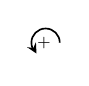
\begin{tikzpicture}[baseline=(char.base)]
    \node(char) at (0,0) {\(\scriptscriptstyle +\)};
    \draw[->, >=stealth, semithick] (0.2,0) arc (0:230:0.18cm);
  \end{tikzpicture}%
}

\usepackage{animate}

\usepackage{calc} % Optional, but helpful for layout

\newcommand{\tikztodo}[3][0.8\textwidth]{%
  \begin{center}
    \fbox{%
      \parbox[c][#2][c]{#1}{%
        \centering
        \textbf{\textcolor{red}{TODO: TikZ Diagram}}\\[0.5em]
        \small #3%
      }%
    }%
  \end{center}%
}

% ============================================================================
% Document Content
% ============================================================================
\begin{document}

\maketitle              % Redefined in the preamble to generate a full frame

\begin{frame}
    \frametitle{Agenda}
    \begingroup
        % Tighten the spacing between paragraphs/TOC lines
        \setlength{\parskip}{0.3em} 
        
        % Optionally tighten the line spacing within an entry
        %\baselineskip=1.2em 
        
        \setcounter{tocdepth}{1} % Show only sections
    \tableofcontents
    \setcounter{tocdepth}{2} % Reset back to default so subsections are tracked
    \endgroup
\end{frame}

\begin{frame}
    \frametitle{Student Learning Outcomes}
    \begin{itemize}[<+- | alert@+>]
        \item[1.]{Create programs in Ladder Logic using the following instructions in an application}
        \item[2.]{Program PLC timers and counters}
    \end{itemize}
\end{frame}

\section{Digital vs. Analog}

\begin{frame}
    \frametitle{Digital Defined}

    \begin{columns}
        \begin{column}{0.48\linewidth}
            \begin{itemize}
                \item Data or signals that have a fixed number of discrete values within their range
                \item Devices that use such data/signals
            \end{itemize}
        \end{column}        
        \begin{column}{0.48\linewidth}
            \begin{figure}
                \centering
                \hexpic[]{0.875\linewidth}{A wall-mounted digital clock with bright red LED numbers displaying the time ten twenty-eight with smaller digits showing eighteen seconds. The clock has a rectangular metal frame and is mounted near the corner of a white ceiling and wall, next to a small white junction box with connecting wires. The glowing red light from the display casts a soft pink hue on the adjacent wall surface.}{../../assets/images/Digital_clock_in_district_court_in_Gliwice,_Silesian_Voivodeship,_Poland,_February_2022}

                {\tiny "Digital clock" by MichalPL, \href{https://creativecommons.org/licenses/by-sa/4.0}{CC BY-SA 4.0}, via \href{https://commons.wikimedia.org/wiki/File:Digital_clock_in_district_court_in_Gliwice,_Silesian_Voivodeship,_Poland,_February_2022.jpg}{Wikimedia Commons}\par}
            \end{figure}
        \end{column}
    \end{columns}
\end{frame}

\begin{frame}
    \frametitle{Digital Signals (1 of 2)}

    \begin{columns}
        \begin{column}{0.48\linewidth}
            \begin{itemize}
                \item \emph{Binary} is a special case of digital--the range is 0-1
                \item All binary signals are digital, not all digital signals are binary
            \end{itemize}
        \end{column}
        \begin{column}{0.48\linewidth}
            \begin{figure}
                \centering
                \resizebox{0.75\linewidth}{!}{
                    \begin{circuitikz}[
    american,
    voltage dir=RP,
    >=latex,
    %>={Latex[length=5mm, width=2mm]},
    alt={}
    ]

    \begin{pgfonlayer}{ft}

        \draw[
            BakerBlack, 
            ultra thick
        ]
        (0,7.5) -- (0,0) -- (4.5,0);
    
        \foreach \y in {1,2,...,7}{

            \pgfmathsetmacro\ylab{\y * 0.5}

            \draw[
                BakerBlack
            ]
            (0.125,\y)
            -- (-0.125,\y)
            node[
                text=BakerBlack,
                left
            ]
            {\ylab};

        }
    \end{pgfonlayer}

    \begin{pgfonlayer}{bg}
    
        \fill[
            draw=LakeBlue,
            fill=LakeBlue,
            fill opacity=0.5,
            thick
        ]
        (0,0)
        -- (0,3)
        -- (1,3)
        -- (1,4)
        -- (2,4)
        -- (2,5)
        -- (3,5)
        -- (3,6)
        -- (4,6)
        -- (4,0)
        -- (0,0);

    \end{pgfonlayer}

    \begin{pgfonlayer}{main}
    
        \fill[
            draw=BakerADARed,
            fill=BakerADARed,
            fill opacity=0.5,
            thick
        ]
        (1,0)
        -- (1,2)
        -- (2,2)
        -- (2,0)
        -- (0,0);

    \end{pgfonlayer}

\end{circuitikz}
                }
            \end{figure}
        \end{column}        
    \end{columns}    
\end{frame}

\begin{frame}
    \frametitle{Digital Signals (2 of 2)}

    \begin{columns}
        \begin{column}{0.48\linewidth}
            \begin{itemize}
                \item Digital signals \emph{can} have decimal points, even a \emph{lot} of decimal points
                \item But they can still only be a fixed number of values
                \item For example this signal can be 2 or 2.5, nothing between
            \end{itemize}
        \end{column}
        \begin{column}{0.48\linewidth}
            \begin{figure}
                \centering
                \resizebox{0.75\linewidth}{!}{
                    \begin{circuitikz}[
    american,
    voltage dir=RP,
    >=latex,
    %>={Latex[length=5mm, width=2mm]},
    alt={}
    ]

    \begin{pgfonlayer}{ft}

        \draw[
            BakerBlack, 
            ultra thick
        ]
        (0,7.5) -- (0,0) -- (4.5,0);
    
        \foreach \y in {1,2,...,7}{

            \pgfmathsetmacro\ylab{\y * 0.5}

            \draw[
                BakerBlack
            ]
            (0.125,\y)
            -- (-0.125,\y)
            node[
                text=BakerBlack,
                left
            ]
            {\ylab};

        }
    \end{pgfonlayer}

    \begin{pgfonlayer}{bg}
    
        \fill[
            draw=LakeBlue,
            fill=LakeBlue,
            fill opacity=0.5,
            thick
        ]
        (0,0)
        -- (0,3)
        -- (1,3)
        -- (1,4)
        -- (2,4)
        -- (2,5)
        -- (3,5)
        -- (3,6)
        -- (4,6)
        -- (4,0)
        -- (0,0);

    \end{pgfonlayer}

    \begin{pgfonlayer}{main}
    
        \fill[
            draw=BakerADARed,
            fill=BakerADARed,
            fill opacity=0.5,
            thick
        ]
        (1,0)
        -- (1,2)
        -- (2,2)
        -- (2,0)
        -- (0,0);

    \end{pgfonlayer}

\end{circuitikz}
                }
            \end{figure}
        \end{column}        
    \end{columns}    
\end{frame}

\begin{frame}
    \frametitle{Analog Defined}

    \begin{columns}
        \begin{column}{0.48\linewidth}
            \begin{itemize}
                \item Data or signals that vary continuously over a range of values
                \item Devices that use this type of data/signal
            \end{itemize}
        \end{column}        
        \begin{column}{0.48\linewidth}
            \begin{figure}
                \centering
                \hexpic[]{0.875\linewidth}{A vertical mercury thermometer mounted on a marble base shaped like a tall trapezoid with a tapered top set against a wooden background. The thermometer features a white face labeled with a capital C at the top for Celsius and numerical markings ranging from below zero to thirty degrees, with orange zeros and black numbers for ten, twenty, and thirty. The glass tube in the center has a reflective metallic bulb at the bottom, and the liquid level rises to indicate a temperature around twenty-one degrees.}{../../assets/images/Mercury_Thermometer}

                {\tiny "Mercury-in-glass thermometer" by Anonimski, \href{https://creativecommons.org/licenses/by-sa/3.0}{CC BY-SA 3.0}, via \href{https://commons.wikimedia.org/wiki/File:Mercury_Thermometer.jpg}{Wikimedia Commons}\par}
            \end{figure}
        \end{column}
    \end{columns}
\end{frame}

\begin{frame}
    \frametitle{Analog Signals}

    \begin{columns}
        \begin{column}{0.48\linewidth}
            \begin{itemize}
                \item Digital signals \emph{can} have decimal points, even a \emph{lot} of decimal points
                \item But they can still only be a fixed number of values
                \item For example this signal can be 2 or 2.5, nothing between
            \end{itemize}
        \end{column}
        \begin{column}{0.48\linewidth}
            \begin{figure}
                \centering
                \resizebox{\linewidth}{!}{
                    \begin{circuitikz}[
    american,
    voltage dir=RP,
    >=latex,
    %>={Latex[length=5mm, width=2mm]},
    alt={}
    ]

    \begin{pgfonlayer}{ft}

        \draw[
            BakerBlack, 
            ultra thick
        ]
        (0,7.5) -- (0,0) -- (6.5,0);
    
        \foreach \y in {1,2,...,7}{

            \pgfmathsetmacro\ylab{\y * 0.5}

            \draw[
                BakerBlack
            ]
            (0.125,\y)
            -- (-0.125,\y)
            node[
                text=BakerBlack,
                left
            ]
            {\ylab};

        }
    \end{pgfonlayer}

    \begin{pgfonlayer}{main}
    
        \fill[
            draw=BakerADARed,
            fill=BakerADARed,
            fill opacity=0.4,
            thick
        ]
        (0,0)
        .. controls (2.5,4) and (4.5,2) ..
        (6,6)
        -- (6,0)
        -- (0,0);

    \end{pgfonlayer}

\end{circuitikz}
                }
            \end{figure}
        \end{column}        
    \end{columns}
\end{frame}

\begin{frame}
    \frametitle{Why Analog?}

    \begin{columns}
        \begin{column}{0.48\linewidth}
            \begin{itemize}
                \item Motors use 69\% of all electricity in the U.S. industrial sector$^1$
                \item Motors running at full speed use more energy than motors running at reduced speed
            \end{itemize}
        \end{column}        
        \begin{column}{0.48\linewidth}
            \begin{figure}
                \centering
                %\hexpic[]{0.875\linewidth}{}{../../assets/images/Ac-elektromotor-robuster-asynchronmotor}

                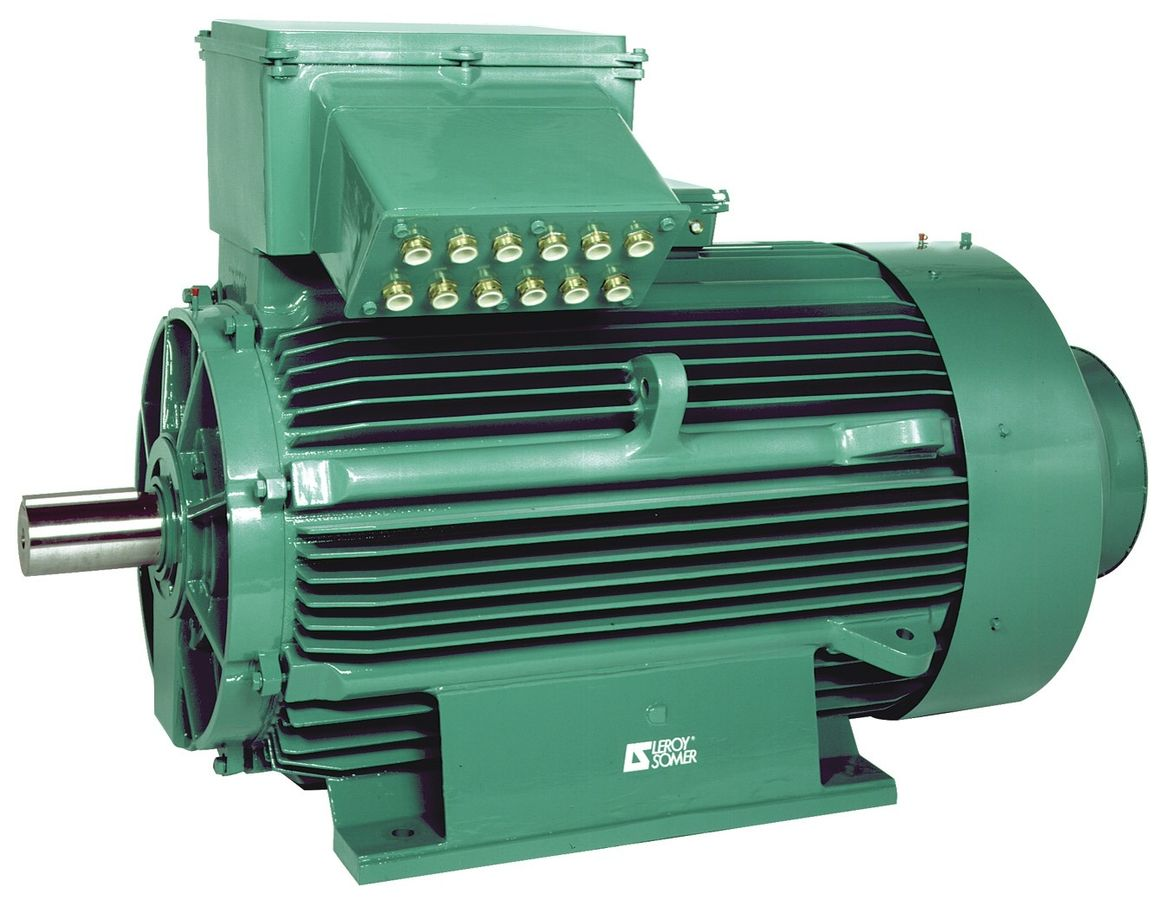
\includegraphics[width=\linewidth]{../../assets/images/Ac-elektromotor-robuster-asynchronmotor}

                {\tiny ``Asynchronous electric motor" by Egzon123, \href{https://creativecommons.org/licenses/by-sa/3.0}{CC BY-SA 3.0}, via \href{https://commons.wikimedia.org/wiki/File:Ac-elektromotor-robuster-asynchronmotor.jpg}{Wikimedia Commons}\par}
            \end{figure}
        \end{column}
    \end{columns}

    \vspace{1em}
    {\scriptsize $^1$Department of Energy, ``Industrial Electric Motor Market Assessment" (2020).\par}
\end{frame}

\begin{frame}
    \frametitle{Controlling Motor Speed}

    \begin{columns}
        \begin{column}{0.48\linewidth}
            \begin{itemize}
                \item When a motor doesn't \emph{need} to run at full speed you \emph{could} use a gearbox\dots
                \item \dots but that doesn't save any energy
            \end{itemize}
        \end{column}        
        \begin{column}{0.48\linewidth}
            \begin{figure}
                \centering
                \hexpic[]{0.875\linewidth}{}{../../assets/images/ZF_Gearbox_Bauma_2004}

                {\tiny ``ZF gearbox at the Bauma trade fair 2004" by Aconcagua, \href{https://creativecommons.org/licenses/by-sa/3.0}{CC BY-SA 3.0}, via \href{https://commons.wikimedia.org/wiki/File:ZF_Gearbox_Bauma_2004.jpg}{Wikimedia Commons}\par}
            \end{figure}
        \end{column}
    \end{columns}
\end{frame}

\begin{frame}
    \frametitle{Saving Motor Energy}

    \begin{columns}
        \begin{column}{0.48\linewidth}
            \begin{itemize}
                \item Save energy (\$) by reducing motor speed
                \item VFDs \emph{always} have an analog input
                \item Most have 2: voltage and current
                \item Can accept either potentiometer or PLC analog output
            \end{itemize}
        \end{column}        
        \begin{column}{0.48\linewidth}
            \begin{figure}
                \centering
                \hexpic[]{0.875\linewidth}{}{../../assets/images/Mitsubishi_frekvenčni_pretvornik}

                {\tiny ``Mitsubishi frequency converter type D700" by Ignac.mihevc at Slovenian Wikipedia, \href{https://creativecommons.org/licenses/by-sa/3.0}{CC BY-SA 3.0}, via \href{https://commons.wikimedia.org/wiki/File:Mitsubishi_frekven\%C4\%8Dni_pretvornik.jpg}{Wikimedia Commons}\par}
            \end{figure}
        \end{column}
    \end{columns}
\end{frame}

\section{Analog Types}

\begin{frame}
    \frametitle{Analog Signal Types}

    \begin{columns}[t]
        \begin{column}{0.48\linewidth}
            \begin{block}{Voltage}
                \begin{itemize}
                    \item \textbf{0 VDC-10 VDC}
                    \item 0 VDC-5 VDC
                    \item -10 VDC-10 VDC
                \end{itemize}
            \end{block}
        \end{column}
        \begin{column}{0.48\linewidth}
            \begin{block}{Current}
                \begin{itemize}
                    \item 0 mA-20 mA
                    \item \textbf{4 mA-20 mA}
                \end{itemize}
            \end{block}
        \end{column}
    \end{columns}
\end{frame}

\begin{frame}
    \frametitle{Which Are the Most Common}

    \centering
    \Large{Which types are the most common?}
\end{frame}

\begin{frame}
    \frametitle{Analog Example}

    \begin{itemize}
        \item Two different analog sensors--identical except for their signal output
        \item Temperature range: 0$^\circ$F-212$^\circ$F
        \item One sensor produces a 0 VDC-10 VDC signal
        \item One sensor produces a 4 mA-20 mA signal
    \end{itemize}
\end{frame}

\begin{frame}
    \frametitle{Analog Scaling (1 of 2)}

    \begin{itemize}
        \item Analog devices will produce an output that directly relates to the property being measured
        \item Almost always linear: 1 V = 3$^\circ$F, 2 V = 6$^\circ$F, 3 V = 9$^\circ$F, etc.
        \item To convert divide the range of the sensor by the range of the analog signal
    \end{itemize}
\end{frame}

\begin{frame}
    \frametitle{Analog Scaling (2 of 2)}

    \begin{itemize}
        \item $212^\circ\text{F} \div 10\,\text{VDC}=21.2^\circ \text{F/V}$
        \item $212^\circ\text{F} \div 16\,\text{mA}=13.25^\circ \text{F/mA}$
        \begin{itemize}
            \item Remember, it starts at 4, the range is only 16
        \end{itemize}
        \item Also remember that analog signals are \emph{analog}--that means they're infinite
        \item These are values per unit, there an infinite number of values between
    \end{itemize}
\end{frame}

\begin{frame}
    \frametitle{Temperature Sensor (1 of 6)}

    \begin{table}
        \centering
        \tagpdfsetup{table/header-rows={1}}
        \begin{tabular}{|c|c|c|c|}
            \hline
            Temp ($^\circ$F) & Volts & Temp ($^\circ$F) & Milliamps\\
            \hline
             -42.40 & 0 & -26.5 & 4\\
             \hline
             -21.20 & 0 & -13.5 & 4\\
             \hline
             \hline
             0 & 0 & 0 & 4\\
             \hline
             21.2 & 1 & 13.25 & 5\\
             \hline
             31.8 & 1.5 & 53 & 8\\
             \hline
             106 & 5 & 106 & 12\\
             \hline
             159 & 7.5 & 159 & 16\\
             \hline
             201.4 & 9.5 & 198.75 & 19\\
             \hline
             212 & 10 & 212 & 20\\
             \hline
             \hline
             233.2 & 10 & 225.25 & 20\\
             \hline
        \end{tabular}
    \end{table}
\end{frame}

\begin{frame}
    \frametitle{Temperature Sensor (2 of 6)}

    \begin{table}
        \centering
        \tagpdfsetup{table/header-rows={1}}
        \begin{tabular}{|c|c|c|c|}
            \hline
            Temp ($^\circ$F) & Volts & Temp ($^\circ$F) & Milliamps\\
            \hline
             -42.40 & 0 & -26.5 & 4\\
             \hline
             -21.20 & 0 & -13.5 & 4\\
             \hline
             \hline
             0 & 0 & 0 & 4\\
             \hline
        \end{tabular}
    \end{table}

    \vspace{1em}
    \centering
    {\footnotesize If the temperature decreases past the bottom of the sensor range the sensor will stay at the bottom value\par}
\end{frame}

\begin{frame}
    \frametitle{Temperature Sensor (3 of 6)}

    \begin{table}
        \centering
        \tagpdfsetup{table/header-rows={1}}
        \begin{tabular}{|c|c|c|c|}
            \hline
            Temp ($^\circ$F) & Volts & Temp ($^\circ$F) & Milliamps\\
             \hline
             212 & 10 & 212 & 20\\
             \hline
             \hline
             233.2 & 10 & 225.25 & 20\\
             \hline
        \end{tabular}
    \end{table}

    \vspace{1em}
    \centering
    {\footnotesize At the exact top of the sensor range the sensor will send out its maximum value\par}
\end{frame}

\begin{frame}
    \frametitle{Temperature Sensor (4 of 6)}

    \begin{table}
        \centering
        \tagpdfsetup{table/header-rows={1}}
        \begin{tabular}{|c|c|c|c|}
            \hline
            Temp ($^\circ$F) & Volts & Temp ($^\circ$F) & Milliamps\\
             \hline
             212 & 10 & 212 & 20\\
             \hline
             \hline
             233.2 & 10 & 225.25 & 20\\
             \hline
        \end{tabular}
    \end{table}

    \vspace{1em}
    \centering
    {\footnotesize The sensor will continue to send out its maximum value for any value above the sensor range\par}
\end{frame}

\begin{frame}
    \frametitle{Temperature Sensor (5 of 6)}

    \begin{table}
        \centering
        \tagpdfsetup{table/header-rows={1}}
        \begin{tabular}{|c|c|c|c|}
            \hline
            Temp ($^\circ$F) & Volts & Temp ($^\circ$F) & Milliamps\\
            \hline
             -42.40 & 0 & -26.5 & 4\\
             \hline
             -21.20 & 0 & -13.5 & 4\\
             \hline
             \hline
             0 & 0 & 0 & 4\\
             \hline
        \end{tabular}
    \end{table}

    \vspace{1em}
    \centering
    {\footnotesize Exactly \emph{at} the bottom of the sensor range a 0 VDC-10 VDC sensor will register 0 VDC\par}
\end{frame}

\begin{frame}
    \frametitle{Temperature Sensor (6 of 6)}

    \begin{table}
        \centering
        \tagpdfsetup{table/header-rows={1}}
        \begin{tabular}{|c|c|c|c|}
            \hline
            Temp ($^\circ$F) & Volts & Temp ($^\circ$F) & Milliamps\\
            \hline
             -42.40 & 0 & -26.5 & 4\\
             \hline
             -21.20 & 0 & -13.5 & 4\\
             \hline
             \hline
             0 & 0 & 0 & 4\\
             \hline
        \end{tabular}
    \end{table}

    \vspace{1em}
    \centering
    {\footnotesize Exactly \emph{at} the bottom of the sensor range a 4 mA-20 mA sensor will register 4 mA\par}
\end{frame}

\begin{frame}
    \frametitle{Which to Pick}

    \centering
    \Large{Which of these is preferred?}
\end{frame}

\begin{frame}
    \frametitle{Analog Signal Selection}

    \begin{columns}[t]
        \begin{column}{0.48\linewidth}
            \begin{block}{0 VDC-10 VDC}
                \begin{itemize}
                    \item Easy unit conversion
                    \item 0 is bottom, 10 is the top
                \end{itemize}
            \end{block}
        \end{column}
        \begin{column}{0.48\linewidth}
            \begin{block}{4 mA-20 mA}
                \begin{itemize}
                    \item Current not as susceptible to noise as voltage
                    \item Easy to diagnose--will \emph{always} return at least 4 mA
                    \item If you ever get a 0 something is wrong
                \end{itemize}
            \end{block}
        \end{column}
    \end{columns}
\end{frame}

\section{Analog Devices}

\begin{frame}
    \frametitle{Analog Inputs}

    \begin{columns}
        \begin{column}{0.48\linewidth}
            \begin{itemize}
                \item Converts physical properties to analog signal
                \item A-to-D converter converts current/voltage to a binary number
                \item Some require external power source
            \end{itemize}
        \end{column}
        \begin{column}{0.48\linewidth}
            \begin{figure}
                \centering
                \hexpic[]{0.875\linewidth}{An industrial temperature sensor lying diagonally on a speckled grey surface. The sensor consists of a long, thin, metallic silver probe extending from a cylindrical gray connection head, which features a round top cover with visible text including PT 100 and Gefran. Four insulated wires, two bright red and two blue, extend out from a threaded port at the top of the connection head.}{../../assets/images/Pt-100_temperature_sensor_with_cables}

                {\tiny "Pt-100 temperature sensor with cables" by Bitjungle, \href{https://creativecommons.org/licenses/by-sa/4.0}{CC BY-SA 4.0}, via \href{https://commons.wikimedia.org/wiki/File:Pt-100_temperature_sensor_with_cables.jpg}{Wikimedia Commons}\par}
            \end{figure}            
        \end{column}
    \end{columns}
\end{frame}

\begin{frame}
    \frametitle{Analog Outputs}

    \begin{columns}
        \begin{column}{0.48\linewidth}
            \begin{itemize}
                \item Converts analog signals to physical properties
                \item A-to-D converter converts analog signal to current/voltage
                \item Some require external power source
            \end{itemize}
        \end{column}
        \begin{column}{0.48\linewidth}
            \begin{figure}
                \centering
                \hexpic[]{0.875\linewidth}{An industrial control valve assembly integrated into a system of stainless steel piping. The valve body at the bottom is connected by flanged joints, supporting a vertical green column topped with a large, rounded blue pneumatic actuator dome. Mounted around the central housing are various components, including a square dark grey Fisher valve positioner box, a black filter regulator, a cylindrical grey module, and two small round pressure gauges on the side. Blue and orange tubing runs between the components against an off-white wall background.}{../../assets/images/Control_valve_with_positioner}

                {\tiny "A Fisher control valve with positioner" by Bitjungle, \href{https://creativecommons.org/licenses/by-sa/4.0}{CC BY-SA 4.0}, via \href{https://commons.wikimedia.org/wiki/File:Control_valve_with_positioner.jpg}{Wikimedia Commons}\par}
            \end{figure}            
        \end{column}
    \end{columns}
\end{frame}

\begin{frame}
    \frametitle{Analog to Digital (A-to-D) Converter}

    \begin{itemize}
        \item Analog \emph{really} is infinite
        \item PLCs (and all computers) are digital--everything is 1's and 0's
        \item A-to-D converters convert the current/voltage to binary
        \item Each bit represents a certain number of volts/amps
    \end{itemize}
\end{frame}

\begin{frame}
    \frametitle{Maximum Analog Value (1 of 2)}

    \begin{itemize}
        \item The maximum value of the binary number from the A-to-D depends on the \emph{bit resolution} of the converter
        \item Let's take the example temperature sensors and plug them into a Micrologix 1000
        \item The Micrologix 1000 has a 10-bit analog resolution
    \end{itemize}
\end{frame}

\begin{frame}
    \frametitle{Maximum Analog Value (2 of 2)}

    \begin{table}
        \centering
        \tagpdfsetup{table/header-rows={1}}
        \begin{tabular}{|c|c|c|c|c|c|c|c|c|c|c|}
            \hline
            Bit & 9 & 8 & 7 & 6 & 5 & 4 & 3 & 2 & 1 & 0\\
            \hline
            Bit Value & 512 & 256 & 128 & 64 & 32 & 16 & 8 & 4 & 2 & 1\\
            \hline
            Total & \textcolor{BakerADARed}{1023} & 511 & 255 & 127 & 63 & 31 & 15 & 7 & 3 & 1\\
            \hline
        \end{tabular}
    \end{table}

    \vspace{1em}
    \centering
    {\footnotesize 1023 is the largest number that can fit in 10 bits\par}
\end{frame}

\begin{frame}
    \frametitle{Analog Resolution}

    \begin{itemize}
        \item The A-to-D has a bit resolution--the number of bits it uses to store the analog conversion
        \item This means that each bit correlates to a specific number of volts/amps 
        \item This \emph{also} means that each bit correlates to a specific real-world value
    \end{itemize}
\end{frame}

\begin{frame}
    \frametitle{Analog Resolution - Volts}

    \begin{itemize}
        \item $10\,\text{V} \div 1023 = 0.009775\,\text{V/bit}$
        \item $21.2^\circ\text{F/V} \times 0.009775\,\text{V/bit} = 0.20723^\circ\text{F/bit}$
        \item This is the \emph{resolution}--this PLC can't see increments smaller than 0.20723$^\circ\text{F}$
    \end{itemize}

    \vspace{1em}

    \begin{table}
        \centering
        \resizebox{\linewidth}{!}{
            \tagpdfsetup{table/header-rows={1}}
            \begin{tabular}{|c|c|c|c|c|c|c|c|c|c|c|}
                \hline
                Bit & 9 & 8 & 7 & 6 & 5 & 4 & 3 & 2 & 1 & 0\\
                \hline
                Volts & 5 & 2.5 & 1.251 & 0.6256 & 0.3128 & 0.1564 & 0.0782 & 0.0391 & 0.019 & 0.0098\\
                \hline
            \end{tabular}
        }
        {\scriptsize Note: table values have been heavily rounded for formatting\par}
    \end{table}
\end{frame}

\begin{frame}
    \frametitle{Analog Resolution - mA}

    \begin{itemize}
        \item $20\,\text{V} \div 1023 = 0.01955\,\text{mA/bit}$
        \item Note: this time we need the \emph{max}--we use 20, not 16
        \item $13.25^\circ\text{F/mA} \times 0.01955\,\text{mA/bit} = 0.259^\circ\text{F/bit}$
        \item This is the \emph{resolution}--this PLC can't see increments smaller than 0.259$^\circ\text{F}$
    \end{itemize}

    \vspace{1em}

    \begin{table}
        \centering
        \resizebox{\linewidth}{!}{
            \tagpdfsetup{table/header-rows={1}}
            \begin{tabular}{|c|c|c|c|c|c|c|c|c|c|c|}
                \hline
                Bit & 9 & 8 & 7 & 6 & 5 & 4 & 3 & 2 & 1 & 0\\
                \hline
                mA & 10 & 5 & 2.502 & 1.251 & 0.6256 & 0.3128 & 0.1564 & 0.0782 & 0.0391 & 0.019\\
                \hline
            \end{tabular}
        }
        {\scriptsize Note: table values have been heavily rounded for formatting\par}
    \end{table}    
\end{frame}

\begin{frame}
    \frametitle{Temperature to Analog 1 (1 of 2)}

    \centering
    \Large{What 10-bit number represents 106$^\circ$F?}

    \vspace{1em}

    \begin{table}
        \centering
        \resizebox{\linewidth}{!}{
            \tagpdfsetup{table/header-rows={1}}
            \begin{tabular}{|c|c|c|c|c|c|c|c|c|c|c|}
                \hline
                Bit & 9 & 8 & 7 & 6 & 5 & 4 & 3 & 2 & 1 & 0\\
                \hline
                Bit Value & 512 & 256 & 128 & 64 & 32 & 16 & 8 & 4 & 2 & 1\\
                \hline
                Volts & 5 & 2.5 & 1.251 & 0.6256 & 0.3128 & 0.1564 & 0.0782 & 0.0391 & 0.019 & 0.0098\\
                \hline
                mA & 10 & 5 & 2.502 & 1.251 & 0.6256 & 0.3128 & 0.1564 & 0.0782 & 0.0391 & 0.019\\
                \hline
            \end{tabular}
        }
        {\scriptsize Note: table values have been heavily rounded for formatting\par}
    \end{table}  
\end{frame}

\begin{frame}
    \frametitle{Temperature to Analog 1 (2 of 2)}

    \begin{itemize}
        \item we know that 106$^\circ$F is half the scale--5 V/12 mA
        \item Start adding up bits to get to those values and do the binary conversion
        \item 0-10 V sensor: 512
        \item 4-20 mA sensor: 614
    \end{itemize}

    \vspace{1em}

    \begin{table}
        \centering
        \resizebox{\linewidth}{!}{
            \tagpdfsetup{table/header-rows={1}}
            \begin{tabular}{|c|c|c|c|c|c|c|c|c|c|c|}
                \hline
                Bit & 9 & 8 & 7 & 6 & 5 & 4 & 3 & 2 & 1 & 0\\
                \hline
                Bit Value & 512 & 256 & 128 & 64 & 32 & 16 & 8 & 4 & 2 & 1\\
                \hline
                Volts & \textcolor{BakerADARed}{5} & 2.5 & 1.251 & 0.6256 & 0.3128 & 0.1564 & 0.0782 & 0.0391 & 0.019 & 0.0098\\
                \hline
                mA & \textcolor{BakerADARed}{10} & 5 & 2.502 & \textcolor{BakerADARed}{1.251} & \textcolor{BakerADARed}{0.6256} & 0.3128 & 0.1564 & \textcolor{BakerADARed}{0.0782} & \textcolor{BakerADARed}{0.0391} & 0.019\\
                \hline
            \end{tabular}
        }
        {\scriptsize Note: table values have been heavily rounded for formatting\par}
    \end{table}  
\end{frame}

\begin{frame}
    \frametitle{Temperature to Analog 2 (1 of 2)}

    \centering
    \Large{What 10-bit number represents 72$^\circ$F?}

    \vspace{1em}

    \begin{table}
        \centering
        \resizebox{\linewidth}{!}{
            \tagpdfsetup{table/header-rows={1}}
            \begin{tabular}{|c|c|c|c|c|c|c|c|c|c|c|}
                \hline
                Bit & 9 & 8 & 7 & 6 & 5 & 4 & 3 & 2 & 1 & 0\\
                \hline
                Bit Value & 512 & 256 & 128 & 64 & 32 & 16 & 8 & 4 & 2 & 1\\
                \hline
                Volts & 5 & 2.5 & 1.251 & 0.6256 & 0.3128 & 0.1564 & 0.0782 & 0.0391 & 0.019 & 0.0098\\
                \hline
                mA & 10 & 5 & 2.502 & 1.251 & 0.6256 & 0.3128 & 0.1564 & 0.0782 & 0.0391 & 0.019\\
                \hline
            \end{tabular}
        }
        {\scriptsize Note: table values have been heavily rounded for formatting\par}
    \end{table}  
\end{frame}

\begin{frame}
    \frametitle{Temperature to Analog 2 (2 of 2)}

    \begin{columns}
        \begin{column}{0.48\linewidth}
            \[
                \begin{aligned}
                    72^\circ\text{F} \div 212^\circ\text{F}&=0.34\\
                    0.34 \times 10\,\text{V}&=3.4\,\text{V}\\
                    3.4\,\text{V}&=342
                \end{aligned}
            \]
        \end{column}
        \begin{column}{0.48\linewidth}
            \[
                \begin{aligned}
                    0.34 \times 16\,\text{mA}&=5.44\,\text{mA}\\
                    5.44\,\text{mA} + 4\,\text{mA} &= 9.44\,\text{mA}\\
                    9.44\,\text{mA}&=481
                \end{aligned}
            \]
        \end{column}
    \end{columns}

    \vspace{1em}

    \begin{table}
        \centering
        \resizebox{\linewidth}{!}{
            \tagpdfsetup{table/header-rows={1}}
            \begin{tabular}{|c|c|c|c|c|c|c|c|c|c|c|}
                \hline
                Bit & 9 & 8 & 7 & 6 & 5 & 4 & 3 & 2 & 1 & 0\\
                \hline
                Bit Value & 512 & 256 & 128 & 64 & 32 & 16 & 8 & 4 & 2 & 1\\
                \hline
                Volts & 5 & \textcolor{BakerADARed}{2.5} & 1.251 & \textcolor{BakerADARed}{0.6256} & 0.3128 & \textcolor{BakerADARed}{0.1564} & 0.0782 & \textcolor{BakerADARed}{0.0391} & \textcolor{BakerADARed}{0.019} & 0.0098\\
                \hline
                mA & 10 & \textcolor{BakerADARed}{5} & \textcolor{BakerADARed}{2.502} & \textcolor{BakerADARed}{1.251} & \textcolor{BakerADARed}{0.6256} & 0.3128 & 0.1564 & 0.0782 & 0.0391 & \textcolor{BakerADARed}{0.019}\\
                \hline
            \end{tabular}
        }
        {\scriptsize Note: table values have been heavily rounded for formatting\par}
    \end{table}  
\end{frame}

\begin{frame}
    \frametitle{Temperature to Analog 3 (1 of 2)}

    \centering
    \Large{What 10-bit number represents 0$^\circ$F?}

    \vspace{1em}

    \begin{table}
        \centering
        \resizebox{\linewidth}{!}{
            \tagpdfsetup{table/header-rows={1}}
            \begin{tabular}{|c|c|c|c|c|c|c|c|c|c|c|}
                \hline
                Bit & 9 & 8 & 7 & 6 & 5 & 4 & 3 & 2 & 1 & 0\\
                \hline
                Bit Value & 512 & 256 & 128 & 64 & 32 & 16 & 8 & 4 & 2 & 1\\
                \hline
                Volts & 5 & 2.5 & 1.251 & 0.6256 & 0.3128 & 0.1564 & 0.0782 & 0.0391 & 0.019 & 0.0098\\
                \hline
                mA & 10 & 5 & 2.502 & 1.251 & 0.6256 & 0.3128 & 0.1564 & 0.0782 & 0.0391 & 0.019\\
                \hline
            \end{tabular}
        }
        {\scriptsize Note: table values have been heavily rounded for formatting\par}
    \end{table}  
\end{frame}

\begin{frame}
    \frametitle{Temperature to Analog 3 (2 of 2)}

    \begin{columns}
        \begin{column}{0.48\linewidth}
            \centering
            For 0-10V, 0 is 0
        \end{column}
        \begin{column}{0.48\linewidth}
            \centering
            0$^\circ$F = 4 mA\\
            4 mA = 204
        \end{column}
    \end{columns}

    \vspace{1em}

    \begin{table}
        \centering
        \resizebox{\linewidth}{!}{
            \tagpdfsetup{table/header-rows={1}}
            \begin{tabular}{|c|c|c|c|c|c|c|c|c|c|c|}
                \hline
                Bit & 9 & 8 & 7 & 6 & 5 & 4 & 3 & 2 & 1 & 0\\
                \hline
                Bit Value & 512 & 256 & 128 & 64 & 32 & 16 & 8 & 4 & 2 & 1\\
                \hline
                Volts & 5 & 2.5 & 1.251 & 0.6256 & 0.3128 & 0.1564 & 0.0782 & 0.0391 & 0.019 & 0.0098\\
                \hline
                mA & 10 & 5 & \textcolor{BakerADARed}{2.502} & \textcolor{BakerADARed}{1.251} & 0.6256 & 0.3128 & \textcolor{BakerADARed}{0.1564} & \textcolor{BakerADARed}{0.0782} & 0.0391 & 0.019\\
                \hline
            \end{tabular}
        }
        {\scriptsize Note: table values have been heavily rounded for formatting\par}
    \end{table}  
\end{frame}

\begin{frame}
    \frametitle{Application}

    \begin{itemize}
        \item In the real world that math almost \emph{never} works
        \item These are all physical devices, no physical device is perfect
        \item It will get you close but usually not close enough
    \end{itemize}
\end{frame}

\subsection{Analog Scaling}

\begin{frame}
    \frametitle{Analog Scaling}

    \begin{itemize}
        \item Analog inputs come in as integers--whole numbers that represent a voltage or current value from the sensor
        \item Most analog cards are 12-bit--the value received by the PLC will be 0-4096
        \item You \emph{can} use this value, but it doesn't mean much to anyone else looking at the code
        \item It is \emph{much} better to scale it to engineering units \emph{before} using it in logic
    \end{itemize}
\end{frame}

\begin{frame}
    \frametitle{Allen-Bradley Scaling}

    \begin{itemize}
        \item Allen-Bradley's preferred method in the Logix 5000 PLCs is to scale the value in the definition of the analog card itself
        \item Not all cards and input devices are equal--if you swap temperature sensors and it's off compared to the old one the scaling needs to be changed
        \item If the scaling is in the card definition, the system needs to be taken offline to change it
        \item Plus, not all manufacturers do it this way--we like ``hardware agnostic" programming methods
    \end{itemize}
\end{frame}

\begin{frame}
    \frametitle{Setting the Scale (1 of 2)}
    \begin{itemize}
        \item Math would tell us the scaling factor would be: $\text{Engineering Units} = \texttt{UnitRange} \times \frac{\texttt{AnalogValue}}{\texttt{MaxValue}}$
        \item This only works \emph{if} the signal starts at 0
        \item It is also only ever going to get you close--not all sensors and cards are equal
        \item Best practice is to actually \emph{measure} the conversion factor
        \item In this case, a spreadsheet is your best friend\dots
    \end{itemize}
\end{frame}

\begin{frame}
    \frametitle{Setting the Scale (2 of 2)}

    \begin{figure}
        \centering
        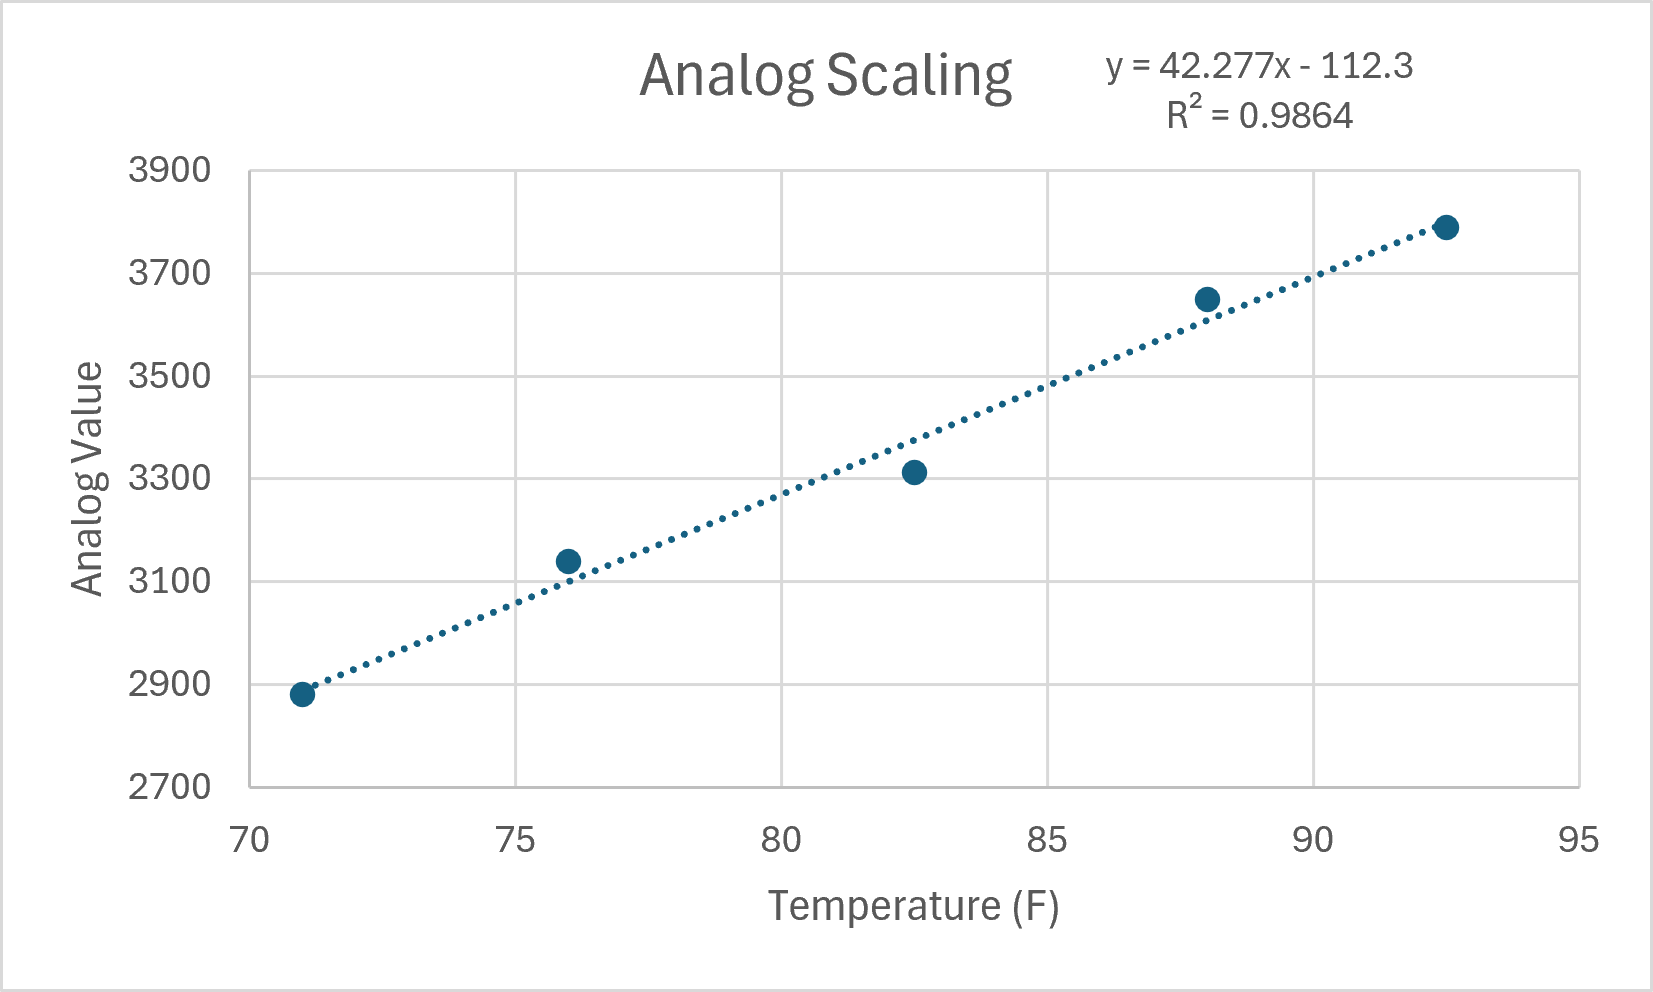
\includegraphics[width=0.5\linewidth, alt={A scatter plot titled Analog Scaling displaying Analog Value on the vertical axis, ranging from 2700 to 3900, against Temperature (F) on the horizontal axis, ranging from 70 to 95. Five dark blue data points show an upward linear trend with a dotted trendline passing through them. The linear regression equation is displayed in the upper right corner as y = 42.277x - 112.3 with an R-squared value of 0.9864.}]{AnalogScaling_Regression.png}

        \vspace{0.5em}
        {\footnotesize Set the sensor to 5-6 known real-world values and read the analog input value. Plot them in a spreadsheet and run a \emph{linear regression}--which the software will do automatically with one click. The regression equation is the scaling factor.\par}
    \end{figure}
\end{frame}

\section{PID Control}

\begin{frame}
    \centering
    {\Huge \textbf{\textcolor{BakerADARed}{Questions?}}}
\end{frame}

\begin{frame}
    \frametitle{Copyright Notice}

    \begin{figure}
        \centering
        
\includegraphics[width=0.625\linewidth, alt={Creative Commons Attribution NonCommercial ShareAlike logo displaying four circular icons arranged horizontally over a black banner. From left to right, the icons feature the CC logo, a person pictogram for Attribution labeled BY below, a slashed dollar sign for NonCommercial labeled NC below, and a counterclockwise circular arrow for ShareAlike labeled SA below.}]{by-nc-sa.png}
    \end{figure}

    \vspace{0.5em}
    \centering
    \PresTitle \textcopyright 2026 by Brad Peirson is licensed under \href{https://creativecommons.org/licenses/by-nc-sa/4.0/}{CC BY-NC-SA 4.0}. To view a copy of this license, visit \href{https://creativecommons.org/licenses/by-nc-sa/4.0/}{https://creativecommons.org/licenses/by-nc-sa/4.0/}
\end{frame}

\end{document}

% \begin{frame}
%     \frametitle{Test Todo}

%     % Usage: \tikztodo[width]{height}{description/notes}
%     \tikztodo[0.7\textwidth]{4cm}{Convert block diagram of feedback loop}
% \end{frame}